Text-aware process prediction aims to utilize unstructured text information in historical event data to improve predictions for unfinished cases.
While many prediction methods have been applied to event data, almost none of them is able to handle textual data.
Nevertheless, much textual information in the context of processes is available, such as business emails, documents, or notes by employees or customers.
These texts in natural language might hold process-critical information and should consequently be considered for process prediction.
However, taking advantage of textual data remains a major challenge since natural language is predominantly context-sensitive and ambiguous \cite{textminingissues}.
A first approach has been presented by \citeauthor{DBLP:conf/bpm/TeinemaaDMF16}, which encodes traces with textual data as vectors, and a random forest classifier is learned for each prefix length \cite{DBLP:conf/bpm/TeinemaaDMF16}.

This chapter presents a novel approach for text-aware process prediction that considers the control flow and additional numerical, categorical and textual data of the process.
An exchangeable text model is used to vectorize textual data and take advantage of potential text-related correlations.
The model aims to capture temporal dependencies between events, seasonal variability, and concept drifts using an event-wise encoding and a sequential LSTM prediction model.
The main application scenario for the model is inside of real-time business process monitoring software, where prediction capabilities for running processes can provide a competitive advantage.

\section{Overview}\label{sec:overview}

The framework is designed to approximate functions $f_\mathrm{a}, f_\mathrm{t}, f_\mathrm{o},$ and $f_\mathrm{c}$ that predict the next activity, next timestamp, case outcome and case cycle time respectively, given any prefix $hd^k(\sigma)$ of length $1 \leq k \leq |\sigma| = n$ of the complete, but unknown trace $\sigma = \langle e_1, \dots, e_{n} \rangle \in \mathcal{E}^+$.
The next activity prediction function $f_\mathrm{a}\colon \mathcal{E}^+ \to \mathcal{A} \cup \{\blacksquare\}$ returns the activity of the next event or an artificial activity $\blacksquare$ if the given trace is already completed, formally:
\begin{align*}
f_\mathrm{a}(hd^k(\sigma)) &= 
\begin{cases}
	\blacksquare& \text{if $k = |\sigma|$} \\
	\pi_\mathcal{A}(\sigma(k+1)) & \text{else} 
\end{cases}
\end{align*}
Furthermore, $f_\mathrm{t} \colon \mathcal{E}^+ \to \mathbb{R}$ returns the time difference between the next event and last event in the prefix to determine the timestamp of the next event:
\begin{align*}
f_\mathrm{t}(hd^k(\sigma)) &=
\begin{cases}
0 & \text{if $k = |\sigma|$} \\
\pi_\mathcal{T}(\sigma(k+1)) - \pi_\mathcal{T}(\sigma(k)) & \text{else} 
\end{cases}
\end{align*}
The case outcome of traces depends on the context of the process.
For example, it can be a binary label describing if the case has been successful or has failed.
In some applications, the case outcome is defined by the activity of the final event of a case.
In that scenario, the outcome function $f_\mathrm{o} \colon \mathcal{E}^+ \to \mathcal{A}$ returns the last activity of the trace:
\begin{align*}
f_\mathrm{o}(hd^k(\sigma)) &= \pi_\mathcal{A}(\sigma(|\sigma|))
\end{align*}
Finally, $f_\mathrm{c} \colon \mathcal{E}^+ \to \mathbb{R}$ returns the total duration of the process, i.e., the time difference between the first and the last event of the trace:
\begin{align*}
f_\mathrm{c}(hd^k(\sigma)) &=  \pi_\mathcal{T}(\sigma(|\sigma|))-  \pi_\mathcal{T}(\sigma(1)).
\end{align*}
All functions are approximated via an LSTM model using historical event log data, i.e., a set of completed traces with full information about the course of the process instances.
The goal is to generalize from the completed traces so that the prediction error is minimized for new, unseen, and incomplete traces.
Due to probabilistic behavior of real-world processes, the prediction accuracy is limited by the randomness of the process behavior.

An overview of the framework is shown in Figure \ref{fig:framework}.
The proposed framework consists of preprocessing, encoding and prediction model components, which operate in an offline and online phase.
In the offline phase, a historical event log with completed traces of a process is used to fit the encoding and prediction components.
Given a historical event log $\eventlog = \{\sigma_1, \dots, \sigma_l\}$ with completed traces, the set of all prefix traces $\eventlog_\mathrm{prefix} = \{ hd^k(\sigma) \mid  \sigma \in \eventlog, 1 \leq k \leq |\sigma|\}$ is computed and each trace is encoded as a sequence of event vectors.

\begin{figure}[!htbp]
	\centering
	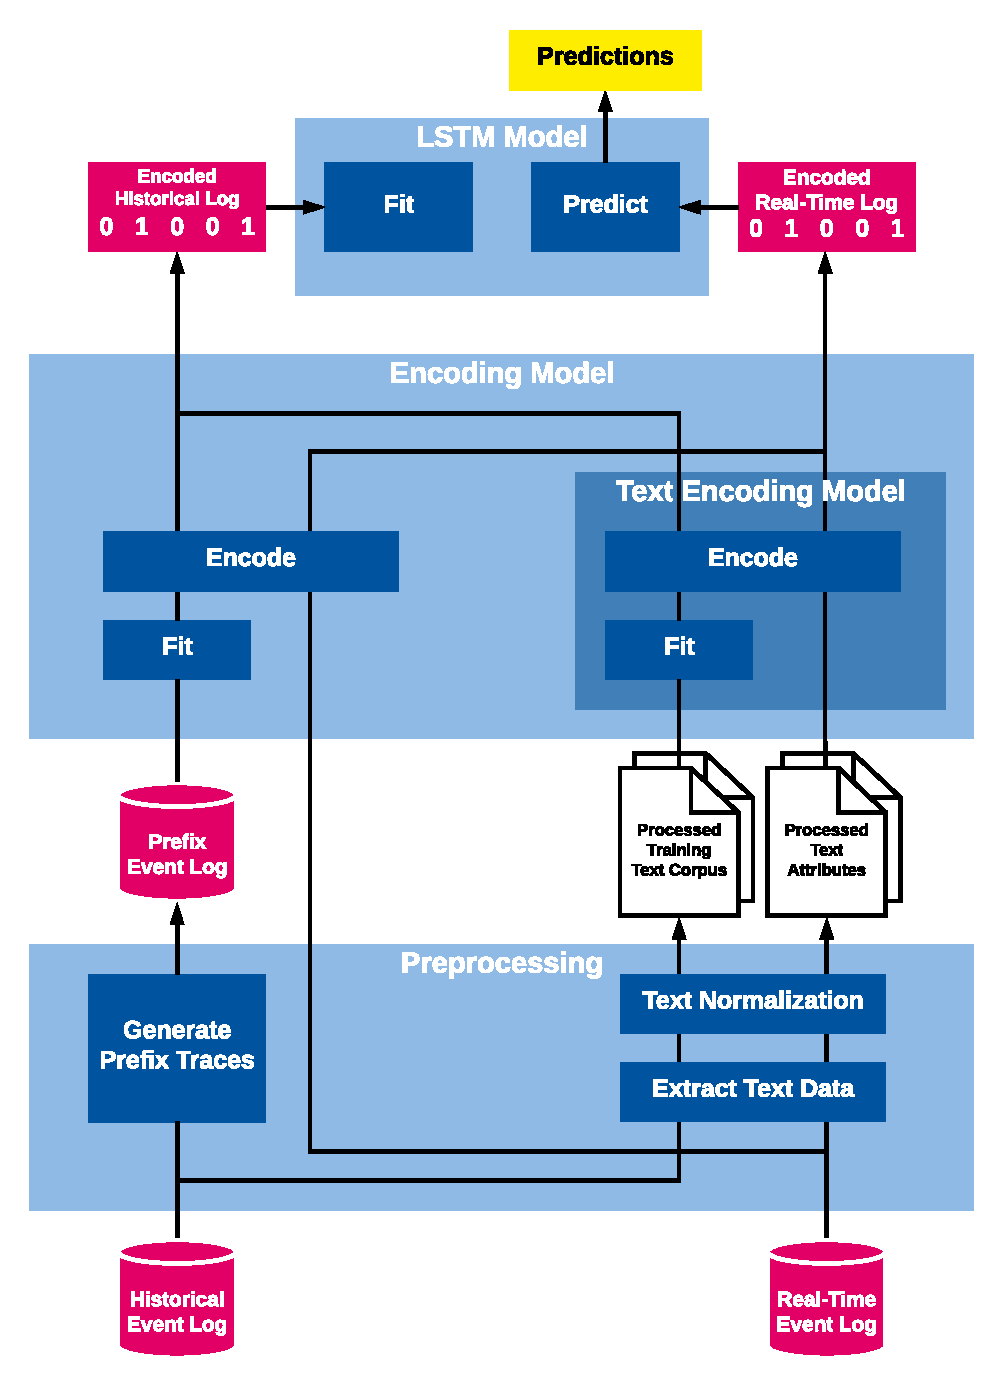
\includegraphics[width=0.8\textwidth]{figures/framework}
	\caption[Overview of the text-aware process prediction model]{Overview of the text-aware process prediction model. Predictions for real-time processes are realized by an LSTM model that is fitted using an encoded representation of all prefixes of the historical event log. The encoding of textual attributes is realized by a text preprocessing pipeline and an exchangeable text encoding model.}
	\label{fig:framework}
\end{figure}

The encoding component distinguishes between categorical and numerical data that can be encoded directly and textual data prepossessed and encoded based on a separate text model.
The text model is an exchangeable component and is fitted to the text corpus, which is extracted from the textual data in the event log $\eventlog$.
Before the textual data of the event log is utilized by the text model, the data is normalized using a text preprocessing pipeline.

Each encoded prefix sequence with its desired prediction target values according to $f_\mathrm{a}, f_\mathrm{t}$, and $f_\mathrm{o}$ corresponds to one training example for an LSTM network that finally realizes the predictions.
The cycle time $f_\mathrm{c}$ is not predicted directly.
Instead, the remaining time is predicted and added to the already elapsed time.
The total number of training examples generated from the log is $\sum_{\sigma \in \eventlog}|\sigma|$, which is exactly the number of events in the log.

In the online phase, the model applies the learned prediction function to predict the activity and time of the next event, the outcome, and cycle time of new, unseen, and unfinished traces in the real-time event log that is monitored by the business process monitoring system.

\section{Event Encoding}\label{sec:event}

In the offline training phase as well as during online prediction, traces are encoded as sequences of event vectors.
The prefix log $\eventlog_\mathrm{prefix}$ is encoded as a training set in the offline phase, while in the online phase running cases are encoded for prediction.
Strictly speaking, an encoding function is realized by the encoding component that transforms prefix traces of length $k$ to vector sequences of the same size, i.e., $encode(\sigma) = \langle \vec{x_1}, \vec{x_2}, \dots, \vec{x_k}\rangle$ with $\sigma = \langle e_1, e_2, \dots, e_k\rangle$ for $k \in \mathbb{N}$.
Each event $e_i$ is encoded as a fixed-length vector using the activity, timestamp and additional categorical, numerical and textual data that is associated with each event.
We assume to have $r \in \mathbb{N}_0$ numerical, $s \in \mathbb{N}_0$ categorical and $u \in \mathbb{N}_0$ textual attributes, i.e., $e_i \in \mathcal{C} \times \mathcal{A}  \times \mathcal{T} \times \mathcal{D}_1^\mathrm{num} \times \dots \times \mathcal{D}_r^\mathrm{num}   \times \mathcal{D}_1^\mathrm{cat}  \times  \dots  \times \mathcal{D}_s^\mathrm{cat}   \times \mathcal{D}_1^\mathrm{text}   \times \dots  \times \mathcal{D}_u^\mathrm{text}$.
Each encoded event vector $\vec{x_i}$ is the concatenation of a set of feature vectors, constructed from the attributes in the event data.
\begin{equation*}
\vec{x_i}=(
\vec{a_i},
\vec{t_i},
d_{i1}^\mathrm{num}, \dots, d_{ir}^\mathrm{num},
\vec{d}_{i1}^\mathrm{cat}, \dots,\vec{d}_{is}^\mathrm{cat},
\vec{d}_{i1}^\mathrm{text}, \dots, \vec{d}_{iu}^\mathrm{text})
\end{equation*}
An overview of each feature vector that is part of the event encoding is provided in Table \ref{tab:features}.
The activity of the event is represented by a vector $\vec{a_i}$ using \textit{one-hot encoding}.
More precisely, given the set of possible activities $\mathcal{A}$, an arbitrary but fixed ordering over $\mathcal{A}$ is introduced with a bijective index function $index_\mathcal{A} \colon \mathcal{A} \to \{1, \dots, |\mathcal{A}|\}$.
Using this function, the activity is encoded as a vector of size $|\mathcal{A}|$, where the component $index_\mathcal{A}(\pi_\mathcal{A}(e))$ has value 1 and all the other components have value 0.
The function $\mathds{1}_\mathcal{A}\colon \mathcal{A} \to \{0,1\}^\mathcal{A}$ is used to describe the realization of such a one-hot encoding transformation for the set of all activities $\mathcal{A}$.
The timestamps of the events are used to compute a six-dimensional vector $\vec{t_i}$ of time-related features, explained in detail in Section \ref*{sec:time}.

\begin{table}[!tbp]
	\renewcommand{\arraystretch}{1.2}
	\setlength\tabcolsep{5pt}
	\begin{tabularx}{\textwidth}{
			>{\hsize=0.6\hsize}X
			>{\hsize=0.8\hsize}X
			>{\hsize=0.6\hsize}X
			>{\hsize=2.0\hsize}X
		}
		\toprule
		\textbf{Feature} \newline \textbf{Vector} & \textbf{Construction} &\textbf{Dimension} &  \textbf{Description} \\
		\midrule
		$\vec{a_i}$ &$\mathds{1}_\mathcal{A}(\pi_\mathcal{A}(e_i))$& $|\mathcal{A}|$& One-hot encoding of the activity. \\
		$\vec{t_i}$ & See Section \ref{sec:time} &6 & Time-based feature vector.\\
		$d_{ij}^\mathrm{num}$ &  $\widehat{\pi_{\mathcal{D}_j^\mathrm{num}}(e_i)} $ &1 & Normalized value of the $j$-th numerical attribute\\
		$\vec{d}_{ij}^\mathrm{cat}$ & $\mathds{1}_{\mathcal{D}_j^{\mathrm{cat}}}(\pi_{\mathcal{D}_j^\mathrm{cat}}(e_i))$&$|\mathcal{D}_j^\mathrm{cat}|$ & One-hot encoding of the $j$-th categorical attribute.\\
		$\vec{d}_{ij}^\mathrm{text}$ & See Section \ref{sec:text} & $z_j$ \newline (parameter) & Fixed-length vectorization of the $j$-th text attribute.\\
		\bottomrule
	\end{tabularx}
	\caption[Feature vectors as part of the event encoding]{Feature vectors as part of the event encoding $\vec{x_i}$ for an event $e_i$.}
	\label{tab:features}
\end{table}

Additional attributes of the events are encoded based on their type, i.e., if they are numerical, categorical, or textual.
Categorical attributes are encoded using one-hot encoding in the same way as the activity, i.e., $\vec{d}_{ij}^\mathrm{cat} = \mathds{1}_{\mathcal{D}_j^{\mathrm{cat}}}(\pi_{\mathcal{D}_j^\mathrm{cat}}(e_i))$ is the vector describing the $j$-th categorical attribute of the $i$-th event.

All additional numerical attributes $\pi_{\mathcal{D}_i^\mathrm{num}} (e_i)$ are scaled to the interval $ [0, 1]$ to improve learning efficiency using min-max normalizing.
The scaling for a numerical attribute $x$ is realized with the transformation
\begin{equation*}
\hat{x} = \dfrac{x-\min(x)}{\max(x) - \min(x)},
\end{equation*}
where $\min(x)$ is the lowest and $\max(x)$ is the highest value $x$ can take.
If the limits are not bounded conceptually, the lowest or highest value of $x$ in the historical event log is used for scaling.

Textual attributes are vectorized via a dedicated text model, which is explained in Section \ref{sec:text}.
The dimensions of the text vectorizations can be tuned individually per attribute using the parameter $z_j$, which is the encoding dimension of the $j$-th textual attribute.

All in all, the encoding of an event $e_i$ results in a vector of size
\begin{equation*}
|\vec{x_i}|= |\mathcal{A}| + r + \sum_{i=1}^{s} |\mathcal{D}_i| + \sum_{j=1}^{u} z_j + 6
\end{equation*}
having $r$ numerical, $s$ categorical and $u$ textual additional attributes (besides activity and timestamp).


\section{Capturing Temporal Dependencies}\label{sec:time}

A set of time-based features is computed from the timestamp data in the event log to profit from the time-related pattern in the process.
As part of the complete encoding $\vec{x}_i$ for an event $e_i$ in a prefix trace $\sigma = \langle e_1, \dots, e_k \rangle$, a time vector $\vec{t_i} = (t_i^1, t_i^2,t_i^3,t_i^4,t_i^5,t_i^6)$ of dimension 6 is computed.
A summary of all time-related features can be seen in Table \ref{tab:time-features}.

\begin{table}[!htbp]
	\centering
	\begin{tabularx}{\textwidth}{l l}
		\toprule
		 \textbf{Feature} & \textbf{Description} \\
		 \midrule
		$t_i^1$ & Normalized time since previous event \\
		$t_i^2$ & Normalized time since case start\\
		$t_i^3$ & Normalized time since first recorded event in the log\\
		$t_i^4$ & Normalized time since midnight (beginning of the day)\\
		$t_i^5$ & Normalized time since last Monday (beginning of the week)\\
		$t_i^6$ & Normalized time since last January 1 00:00 (beginning of the year)\\
		\bottomrule
	\end{tabularx}
	\caption[Time-based features as part of the event encoding]{Time-based features as part of event encoding $\vec{x_i}$.}
	\label{tab:time-features}
\end{table}

Using these features, time-related correlations can be captured and utilized for prediction.
The feature $t_i^1$ describes the time difference between the current event $e_i$ and previous event $e_{i-1}$, while $t_i^2$ gives the time difference between the current event and the first event of the case $e_1$, i.e. the time since the start of the case.
Furthermore, $t_i^3$ is the time difference between the current event and the first event that is recorded in the log.
This feature indicates the absolute time position of an event in the recorded data.
This information is important to detect concept drifts \cite{DBLP:journals/tnn/BoseAZP14} in the process.
Most real-world processes are not static, i.e., the behavior of the process changes over time.
For example, in earlier process executions customers might have been informed by a letter, whereas in more recent cases, customers are messaged using email or app notifications.
Therefore, the knowledge about the event’s absolute time can be used to relate cases in similar periods of time.

The features $t_i^4, t_i^5$ and $t_i^6$ describe the event’s time in relation to the beginning of the day, week, and year.
They are used to capture daily, weekly, and seasonal trends.
For example, some activities might only be executed during office hours or before the weekend.
Also, many businesses expect seasonally fluctuating demand; for example a booking platform for vacation usually has many more customers in summer, affecting the process execution in many ways.
Each feature $t_i^1, \dots, t_i^6$ is min-max normalized such that $t_i^j \in [0,1]$ for $j \in [6]$.

\section{Text Vectorization}\label{sec:text}

In order to prepare the textual data of the event log for a prediction model, the texts have to be encoded in a compact, finite, and useful numerical vector representation using a text model.
Useful in that context means that texts with similar semantic meanings should also have similar representations.
The vector representation of textual data is an important task in \textit{Natural Language Processing} (NLP) \cite{DBLP:books/daglib/0001548}.
Extracting the meaning of textual information remains a challenge even for humans because textual data is unstructured, language-dependent, and domain-specific.
Many words are ambiguous; for example, the word \enquote{apple} might denote a fruit or a global technology company.
In addition, grammatical variations and the importance of context in language makes extracting the semantic meaning even more difficult for computers.

In this setting, the text vectorization for textual attributes is realized in a two-step procedure.
First, all textual data associated with the events in the corresponding textual attribute is collected in a so-called \textit{text corpus}.
Each document in the text corpus is then preprocessed in order to filter out linguistic noise or useless information.
This step is called \textit{text normalization}  \cite{DBLP:books/lib/JurafskyM09}.
Finally, the normalized text corpus is used to build up a \textit{vocabulary}, and a text vectorization technique is applied to encode the text of the attribute into a fixed-length vector.
The vocabulary of a text corpus is a set $V$ of all relevant words that appear after preprocessing in the corpus, which is indexed by a bijective index function $index_V \colon V \to \{1, 2, \dots, |V|\}$.
As text vectorization techniques, the \textit{Bag of Words}, \textit{Bag of N-Grams}, \textit{Paragraph Vector}, and \textit{Latent Dirichlet Allocation} text models are considered, which are discussed in more detail in Sections \ref{sec:bow} through \ref{sec:lda}.

\subsection{Text Normalization}

In the text normalization step each document of the text corpus is transformed by a preprocessing pipeline, which performs the following four steps:
\begin{enumerate} 
	\item Letters are converted to lowercase.
	\item The document is tokenized (i.e., split) by word.
	\item Each word is lemmatized.
	\item Stop words are filtered out.
\end{enumerate}
The first step eliminates all capital letters in the text.
In the tokenization step, a document is split up into a sequence of words.
Each word is then lemmatized, i.e., it is converted to its canonical form.
The idea is to unify words that have a very similar meaning and filter out grammatical variations.
For example, the words   \enquote{go}, \enquote{going}, \enquote{goes}, \enquote{gone} and   \enquote{went} are all transformed to the basic form   \enquote{go}.
Lemmatization significantly reduces the complexity of textual data while accepting a hopefully small loss of information.

\begin{table}[!htbp]
	\begin{tabularx}{\textwidth}{l l p{9.8cm}}
		\toprule
		\textbf{Step} & \textbf{Transformation} & \textbf{Example Document}                                                       \\ \midrule
		0             & Original       &   \enquote{The patient has been diagnosed with high blood pressure.} \\
		1             & Lowercase               &   \enquote{the patient has been diagnosed with high blood pressure.} \\
		2 & Tokenization  & $\langle$\enquote{the}, \enquote{patient}, \enquote{has}, \enquote{been}, \enquote{diagnosed}, \enquote{with}, \enquote{high}, \enquote{blood}, \enquote{pressure}, \enquote{.}$\rangle$ \\
		3 & Lemmatization & $\langle$\enquote{the}, \enquote{patient}, \enquote{have},  \enquote{be}, \enquote{diagnose}, \enquote{with},  \enquote{high}, \enquote{blood}, \enquote{pressure}, \enquote{.}$\rangle$  \\
		4             & Stop word filtering     & $\langle$\enquote{patient}, \enquote{diagnose}, \enquote{high}, \enquote{blood}, \enquote{pressure}$\rangle$ \\ \bottomrule
	\end{tabularx}
	\caption[Text preprocessing transformation of an example document]{Text preprocessing transformation of an example document containing a single sentence.}
	\label{tab:text-preprocessing}
\end{table}

Ultimately, all stop words are filtered out of each document.
Stop words are words with low information value like \enquote{the},  \enquote{a},  \enquote{of} or  \enquote{here}.
Stop word lists are language- and context-dependent and can be more or less aggressive at filtering.
Usually, they contains articles, auxiliary verbs, prepositions, and generic verbs like \enquote{be} and \enquote{have}.
In addition, punctuation marks and numerical symbols are excluded.
An example application of the text normalization pipeline is shown in Table \ref{tab:text-preprocessing}.
Using the corpus of normalized documents (i.e., texts), a text model is fitted in the offline phase to construct the vocabulary and realize the encoding of the textual attributes.
In the following, four different text models are presented that are suitable to construct vector representations of documents.

\subsection{Bag of Words}\label{sec:bow}

The \textit{Bag of Words} (BoW) model is a simple text model, representing documents based on the \textit{term frequencies} of its words while ignoring their order \cite{harris1954distributional}.
Given the learned vocabulary $V$, a document is represented by a vector of size $|V|$, where the $i$-th component gives the number of occurrences in the document of the word indexed with $i$ in the vocabulary.

Since this approach does not reflect the prior distributions of words in the corpus, i.e., how likely certain words appear in a document in general, the term frequencies are usually normalized by the so-called \textit{inverse document frequency} (idf) of a word.
The inverse document frequency indicates the specificity of a word in the corpus and is computed by dividing the total number of documents by the number of documents that contain the specific word and scaling that value logarithmically.
The resulting value is the tf-idf score of a word in a document.

The Bag of Words model is easy to build and effective for certain applications but limited in several ways.
First, the model completely ignores the order of words, which is often crucial for understanding the semantic meaning.
For example, the sentences  \enquote{The patient’s health state went from stable to critical.} and  \enquote{The patient’s health state went from critical to stable.} would result in the same vector representation, while the meaning is clearly the opposite.
Second, the vector representations are sparse and of high dimensionality, since they depend on the size of the vocabulary.
However, the dimension can be reduced by limiting the size of the vocabulary.
For example, words that rarely appear in the corpus can be excluded from the vocabulary.
Unseen words that appear during online prediction and are not part of the learned vocabulary are not considered.

\subsection{Bag of N-Grams}

The \textit{Bag of N-Grams} (BoNG) model is a generalization of the Bag of Words model, which addresses the latter’s missing word order awareness.
Instead of single words, the vocabulary consists of $n$-tuples of words that appear consecutive in the documents.
The unigram model ($n=1$) is equivalent to the BoW model.
For the bigram model ($n=2$), the vocabulary consists of pairs of words that appear next to each other in the documents.
For example, for the preprocessed document $\langle$\enquote{patient},  \enquote{diagnose},  \enquote{high},  \enquote{blood},  \enquote{pressure}$\rangle$, the pairs (\enquote{patient},  \enquote{diagnose}), (\enquote{diagnose},  \enquote{high}), (\enquote{high},  \enquote{blood}) and (\enquote{blood},  \enquote{pressure}) are added the vocabulary.
For $n>2$ $n$-tuples are generated accordingly.
The feature vector is constructed by computing the tf-idf score for each vocabulary entry, like in the BoW model.

Compared to the BoW model, $n$-grams also take the order of words into account, which is beneficial in many scenarios.
However, the vocabulary size is usually even larger than in the BoW model.
In order to generate more compact vectors, distributed text representations are needed for larger text corpora and vocabularies.

\subsection{Paragraph Vector}

The \textit{Paragraph Vector} model (also known as \textit{Doc2Vec}), originally presented by \citeauthor{DBLP:conf/icml/LeM14} in \citeyear{DBLP:conf/icml/LeM14}, is an unsupervised algorithm that learns distributed fixed length vector representations for documents of variable length using a simple feedforward neural network \cite{DBLP:conf/icml/LeM14}.
The idea is inspired by the word embedding model presented by \citeauthor{DBLP:journals/jmlr/BengioDVJ03} \cite{DBLP:journals/jmlr/BengioDVJ03}, which can learn distributed fixed-length vector representations for words.
In this model, words are mapped to vectors, trained to predict words from their context, i.e., words that appear before or after the target word in the training documents.
Several variants of this approach exist, notably the \textit{Continuous Bag of Words} model, which ignores the order of the words in the context, and the \textit{Continuous Skip-gram} model, which predicts the skip-gram context for a word vector (also known as \textit{Word2Vec}) \cite{DBLP:journals/corr/abs-1301-3781}.

\begin{figure}[!htbp]
	\centering
	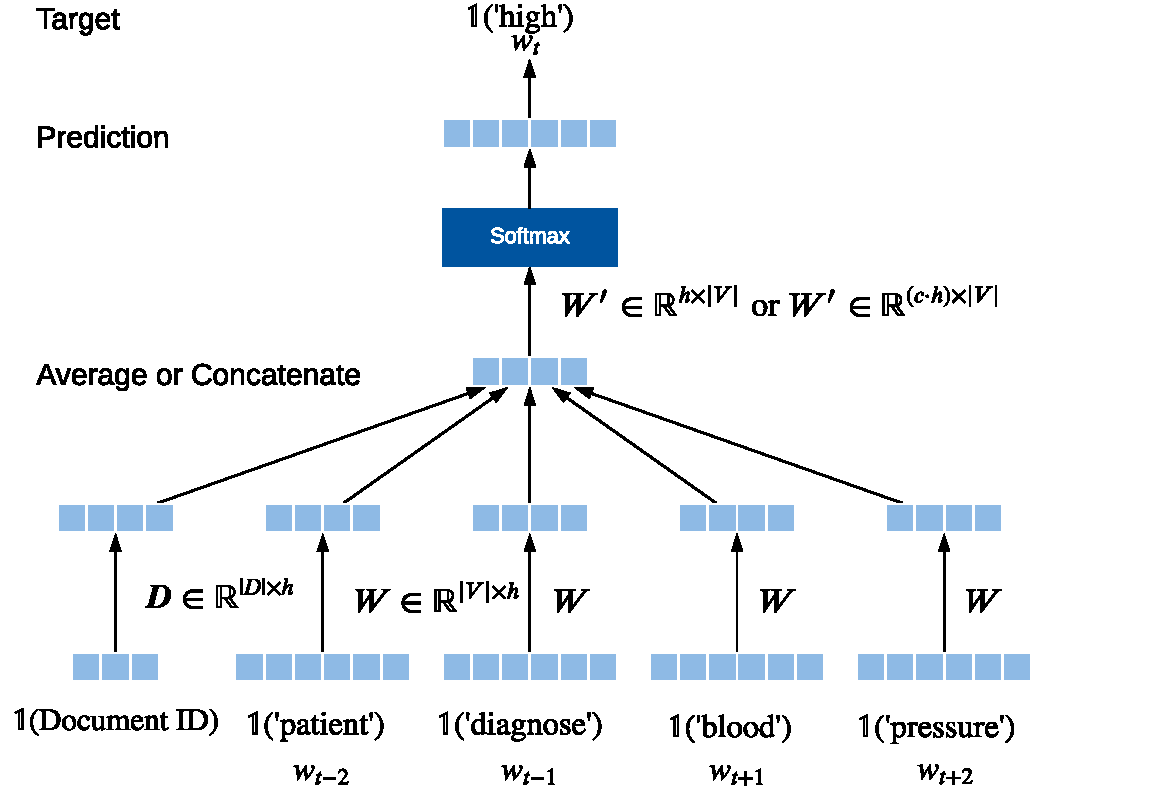
\includegraphics[width=\textwidth]{figures/paragraph-vector}
	\caption[Paragraph Vector model]{The Paragraph Vector model in the distributed memory variant (PV-DM) is a neural network that is designed to predict a word $w_t$ from its context ($w_{t-2}, w_{t-1}, w_{t+1}, w_{t+2}$) and derives fixed-length representation of documents and words via the learned matrices $\vec{D}$ and $\vec{W}$. The dimension of the word and document representations are defined a priori.}
	\label{fig:paragraph-vector}
\end{figure}

The core idea of the Paragraph Vector model is to extend the model introduced in \cite{DBLP:journals/jmlr/BengioDVJ03} in such a way that an additional document (i.e., paragraph) vector is trained together with the word vectors, so that it is unique for each document.
Fig. \ref{fig:paragraph-vector} shows the architecture of the distributed memory variant of the Paragraph Vector model (PV-DM).
It is realized by a neural network, which takes one-hot encoded words and a one-hot encoded document ID as input.
These are mapped to vector representation via weight matrices $\vec{D}$ and $\vec{W}$, which are learned during training with gradient descent.
The distributed representations are then averaged or concatenated to a vector to predict the one-hot encoded target word using another mapping $\vec{W'}$ and a softmax activation function.
The training set is constructed using a sliding window over every document, such that the input is the context of the target word and the document ID.
After training, each column in $\vec{D}$ represents the distributed encoding of the corresponding document.

The network is also able to learn a representation for unseen documents through an inference step.
In this phase, the word matrix $\vec{W}$ and the prediction matrix $\vec{W'}$ are fixed, and only the document vector is trained.
The paragraph vector model tends to perform better than non-distributed models; however, since new documents are vectorized via inference, a bigger training corpus of documents is usually required.

\subsection{Latent Dirichlet Allocation}\label{sec:lda}

The \textit{Latent Dirichlet Allocation} (LDA) presented by \citeauthor{DBLP:journals/jmlr/BleiNJ03} in \citeyear{DBLP:journals/jmlr/BleiNJ03} \cite{DBLP:journals/jmlr/BleiNJ03} is a generative statistical text model, representing documents as a mixture of a small and fixed number of topics.
Topics are defined by a probability distribution over all words in the vocabulary and are also learned by the model in an unsupervised manner.
The underlying assumption of the LDA model is that the documents were created by a statistical process that sampled the words of the document from sampled topics.
A document is encoded as a vector, whose dimension is equal to the number of topics and each component indicates the probability that the corresponding topic distribution was chosen to sample a word in the document.
The distributions and, therefore, document encodings, can be learned with statistical inference algorithms like Monte Carlo Simulation, Variational Bayes or maximum likelihood estimation using the words of each document.
Compared to the other text models, LDA can generate very compact document encodings since the documents are only described by their degree of affiliation to each topic.
Similar to the BoW model, LDA does not consider the order of words in the document, which can be disadvantageous for some text corpora.

\section{Network Architecture and Training}
The encoded historical prefix event log is used to fit an LSTM model.
The LSTM network is designed to be trained with all prediction targets (next activity, next event time, case outcome and case cycle time) together in order to benefit from their correlations.
In the basic variant, the network consists of an input layer, a shared LSTM layer, a specialized LSTM layer for each prediction target, and a fully connected output layer for each target.
Furthermore, layer normalization \cite{DBLP:journals/corr/BaKH16} can be applied after each LSTM layer, which standardizes the hidden output to speed up the training convergence.
The network architecture is shown in Figure \ref{fig:network}.
Note that the LSTM layers in the figure are unrolled in time, i.e., the same layer is displayed once for every time step.

\begin{figure}[!htbp]
	\centering
	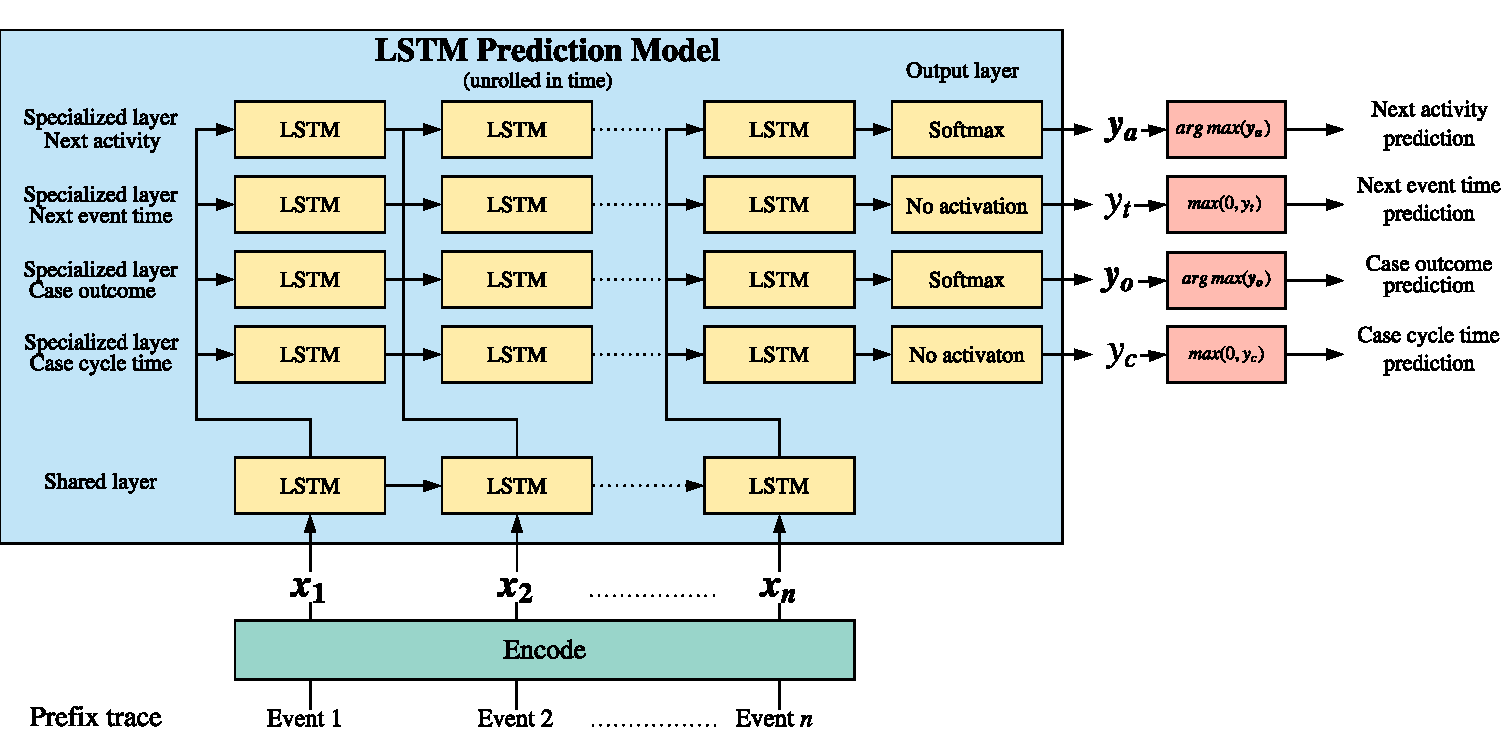
\includegraphics[width=\textwidth]{figures/network}
	\caption[LSTM model architecture for text-aware process prediction]{LSTM model architecture to simultaneously predict the next activity $(\vec{y_a})$, next event time $(y_t)$, case outcome $(\vec{y_o})$ and case cycle time $(y_c)$ for an encoded prefix trace $\vec{x_1}, \vec{x_2}, \dots, \vec{x_k}$.}
	\label{fig:network}
\end{figure}

The fully connected output layer uses a softmax activation function for the next activity and case outcome prediction to estimate the probability for each target value.
The softmax function normalizes a vector of real numbers into another vector of the same dimension, such that all components are in the interval [0,1], and the sum of all components is equal to 1.
Hence, the transformed vector can be interpreted as a probability distribution while keeping the vector’s original proportions.
The softmax function is described with
\begin{equation*}\label{key}
	\text{Softmax}(\vec{x})_i = \frac{\exp(x_i)}{\sum_{j=1}^{n} \exp(x_j)}  \qquad \text{for} \, i = 1, \dots, n \text{ and } \vec{x}=(x_1, \dots, x_n) \in \mathbb{R}^n.
\end{equation*}
The whole training set of encoded prefix traces is represented for efficiency by a 3-dimensional matrix of real values, where the three dimensions specify the prefix traces, the events per prefix trace, and the features per event.
Since the prefix traces have different lengths, shorter traces are pre-padded \cite{DBLP:journals/corr/abs-1903-07288} with zero vectors.
Hence, a prefix trace of encoded events $\vec{x_1}, \vec{x_2}, \dots, \vec{x_n}$  is represented in the training set by a 2-dimensional matrix $(\mathbf{0}, \dots, \mathbf{0},\vec{x_1}, \vec{x_2}, \dots, \vec{x_n})$, such that the zero vectors fill up shorter traces to the length of the longest trace in the training set.
All prefix traces together form a 3-dimensional training matrix.

The training is realized using a learning algorithm based on stochastic gradient descent and backpropagation through time (BPTT), which updates the weights of the network using the update rules of the Adam optimizer with Nesterov momentum \cite{dozat2016incorporating}.
The loss for numerical prediction values $\hat{y}$ and the true value $y$ is the absolute error $\text{AE}(\hat{y},y)=|\hat{y} - y|$, while the loss for categorical prediction values is computed using the categorical cross-entropy error $\text{CE}(\vec{\hat{y}}, \vec{y}) = - \sum_{i=1}^{k} y_i \cdot \log \hat{y}_i$.

\section{Predictive Business Processing Monitoring}

During online business process monitoring, predictions are realized by a forward-pass of the encoded, incompleted traces through the LSTM model.
The component with the highest value of the softmax outputs for the next activity $(\vec{y_a})$ and the case outcome $(\vec{y_o})$ indicates the categorical prediction.
The output values for the next event time $(y_t)$ and case duration  $(y_c)$ are clipped to 0 for negative outputs and the normalization is reverted to compute the final prediction value.

With every new event registered by the business process monitoring system, the prediction can be updated with another forward-pass through the model.
This guarantees a continuous forward-projection on running process instances which is updated whenever new information in the form of new events becomes available.
By predicting the timestamp and activity of the next event in an iterative way, the complete future path of the running process instance can be predicted.
The trace of a process instance is assumed to be completed when the model predicts the artificial $\blacksquare$ activity.
With this technique, the model can indirectly predict the completeness of a case.